%-A Two-Qubit Quantum Processor
%-Building Blocks: Single Qubit Gates, Qubit Readout, Two-Qubit Gate
%-Implementation
%-Frequency Tunability of the Qubits
%  -Decoherence Times
%-Characterization of the Readout
%  -Readout Errors
%-Single Qubit Gates: Tune-Up & Characterization
%-2 Qubit Gate: Tune-Up & Characterization
%-Tests of Entanglement
%  -Entanglement Witnesses
%  -Bell's Inequality
%-2 Qubit Algorithms
%-Grover's Search Algorithm:
%   -Introduction & Background
%   -Implementation
%   -Measurements
%   -Error Analysis
%   -Conclusions

\chapter{Realizing a Two-Qubit Processor}

This chapter discusses the main experimental results of this thesis. We start by discussing the implementation of a superconducting two-qubit processor, discussing the characteristics of the Transmon qubits used in the processor, the readout scheme, single-qubit manipulation, two-qubit gates as well as the experimental procedures used for quantum state and quantum process tomography. The last section of this chapter will discuss the implementation of a quantum algorithm -- so called Grover search algorithm -- using our two-qubit processor and the demonstration of quantum speed-up achieved with our system.

%-Discuss all the experiments performed during the PhD thesis.

\section{Introduction \& Motivation}

\begin{figure}[ht!]
  \centering
	\includegraphics[width=1.\textwidth]{"./material/figures/2-qubit-processor/processor schematic"}
	\caption[Circuit schematic of the two-qubit processor]{The circuit schematic of the two-qubit processor used in this work. Shown are the two Transmon qubits in green, the drive and readout circuit in blue, the fast flux lines in red and the coupling capacitance in magenta.}
	\label{fig:2_qubit_chip_circuit_diagram}
\end{figure}

As discussed in the introduction, the most simple, usable quantum processor contains two qubits that are coupled by an universal two-qubit gate and which in addition can be manipulated and read out individually. We realized such a two-qubit processor using two Transmon qubits, coupled through a fixed capacitance and readout out by individual single-shot readout of the JBA type. The circuit diagram of our processor is shown in fig. \ref{fig:2_qubit_chip_circuit_diagram}, showing the qubits, the drive and readout circuit and the coupling element between them. The following sections we'll discuss the parameters of individual parts of the processor.

\section{Qubit Design}

The parameters of the sample have been chosen in accordance to various design constraints of the qubit processor. For the qubits, the main design goals were high coherence time, good frequency tunability and fast drivability. As we will show later, the coherence time of the qubit is limited by relaxation to the ground state and coupling to external noise sources. The relaxation component of the Transmon qubit is ultimately limited by internal losses of the Josephson junction but usually is bound by coupling to the electromagnetic environment, as will be discussed later. The frequency tunability is important for the realization of fast two-qubit gates but can also limit the relaxation and coherence time of the qubit by coupling to external noise sources. The drivability speed on the other hand is limited by the anharmonicity of the qubit, which can however not be increased arbitrarily since it will make the qubit sensitive to charge noise when chosen too high. For the readout, the main design goals were readout speed and fidelity. The speed of the readout is limited by the quality factor of the readout resonator, which however also can induce qubit relaxation through the Purcell effect and may therefore not be chosen too small.

In the following paragraphs we'll therefore discuss the parameter design for our two-qubit processor and analyze the sample parameters that have been obtained.

\section{Readout Design}

\section{Processor Fabrication}

In this section we will discuss the fabrication of the two-qubit processor realized in this work.

\chapter{Measurement Setup}

\begin{figure}[ht!]
	\centering
		\includegraphics[width=1.\textwidth]{"./material/figures/2-qubit-processor/measurement setup"}
	\caption[The measurement setup used for the two-qubit experiments]{The measurement setup used for the two-qubit experiments. Exactly the same drive and readout scheme is used for both qubits with phase-locked microwave sources and arbitrary waveform generators.}
	\label{fig:MeasurementSetup}
\end{figure}

Fig. \ref{fig:MeasurementSetup} show the measurement setup used for the two-qubit experiments. The different signal and measurement lines as well as the room-temperature and cryogenic microwave components used in our experiments will be described in the following paragraphs.

In this section we discuss the details of the measurement setup used to perform the two-qubit experiments presented in this thesis. All experiments have been performed in a custum-built dilution cryostat at $< 40 \; \mathrm{mK}$ using a cryogenic microwave signal generation and measurement chain. The individual components of this setup will be discussed in the following sections.

\section{Sample Holder \& PCB}

The qubit chip is first glued to a high-frequency PCB \todo{add substrate material details}, then wirebonds are used to connect the groundplane and the center conductors of the on-chip transmission lines to their counterparts on the PCB. Finally, additional bond wires connect isolated ground planes on-chip. The realization of a good and uniform groundplane on the qubit chip and around is very important to supress unwanted resonance modes that can be created when the connection between isolated ground planes is not good enough \todo{Add references e.g. to Schuster's thesis}. The mounted chip on the PCB is then placed in a Copper or Aluminium sample holder which fully encloses the PCB and serves to reduce unwanted couplings to the environment. The coplanar waveguides on the PCB are connected to Mini-SMP cables through a set of connectors that are soldered on the PCB.

\section{Cryogenic Wiring}

For the transmission of microwave signals to our sample we use various types of transmission lines suited for room-temperature and cryogenic application. The main goal of the input lines is to provide adequate signal transmission without introducing too much thermal conductance to the system. For the signal lines that carry the measurement signal from the sample we use superconducting cables \todo{add type} and low-resistance copper cables. In addition, we use superconducting bifilar cables for the DC bias of our magnetic coils. The qubit and fluxline input lines are attenuated and filtered at several stages of the cryostat to reduce signal noise.

\section{Signal Generation \& Acquisition}

Here we discuss the generation and acquisition of the different signals used to manipulate and read out our quantum processor. The experiments that have been performed require the generation, measurement and demodulation of microwave signals, the generation of fast flux control pulses and the application of DC currents to our magnetic coils.

\subsection{Microwave Sideband Mixing}

For qubit manipulation it is often advantageous to use single-sideband mixing for driving the qubit since it can provide higher ON/OFF ratios for microwave pulses and allow the driving of higher qubit-levels using a single, phase-coherent microwave source. To realize this, we use IQ mixers (Hittite \todo{Add exact type number}) that we drive with a continous single-frequency microwave tone and two time-synchronized fast control signals generated by an arbitrary waveform generator (Tektronix AWG5014b). When feeding a signal $LO(t) = i_0 \cos{(\omega_{rf} t )}$ to the LO port of the mixer and two signals $I(t)$, $Q(t)$ to the I and Q ports of the mixer one obtains a signal

\begin{equation}
RF(t) = I(t)\cos{(\omega_{rf} t)}+Q(t)\sin{(\omega_{rf} t)} \label{eq:iqMixer}
\end{equation}

at the LO port of the mixer. Since the IQ mixer that we use is a passive, reciprocal device one can as well feed two input signals to the LO and RF ports and obtain the demodulated signal quadratures at the I and Q ports, a technique that we'll make use of for our qubit readout scheme.

Commercially available IQ mixers often deviate from the ideal behavior as given by eq. (\ref{eq:iqMixer}). Typical imperfections include large insertion losses --i.e. loss of signal power between the different ports of the mixer--, RF signal leakage at zero IQ-input and frequency-dependent phase and amplitude errors of the mixed sideband signals. In order to achieve reliable single-qubit operations we need to correct the signal leakage and quadrature-specific amplitude and phase errors. The signal leakage causes a small part of the LO signal to leak through to the RF port even when the IQ inputs are zeroed. This leakage can be compensated by adding center-frequency $\omega_c$ dependent DC offset voltages to the IQ ports. The appropriate offset voltages can be determined by applying a continuous input signal at a frequency $\omega_c$ to the LO port of the mixer and minimizing the signal power at the RF port by varying the IQ offset voltages. To correct the sideband amplitude and phase errors we apply another correction procedure that we outline here. First, for the signals at the IQ inputs of the mixer we introduce the notation

\begin{equation}
A(t) = I(t)+iQ(t) = a(t)\exp{(-i\phi(t))}
\end{equation}

We consider an IQ signal at a single sideband frequency $\omega_{sb}$ and at fixed complex amplitude $a(t) = a = a_0\exp{(i\phi_0)}$ such that $A(t) = a\exp{(-i \omega_{sb} t)}$. The effect of the gain and phase imperfections of the IQ mixers can then be modeled by assuming that the mixer adds another IQ signal $\epsilon(\omega_{sb},\omega_c)A^*(t)$ at the mirrored sideband frequency $-\omega_{sb}$. We can correct this unwanted signal by adding a small correction $c(\omega_{sb},\omega_c)A^*(t)$ to our IQ input signal. The correction coefficient $c(\omega_{sb},\omega_c)$ usually depends both on the carrier frequency $\omega_c$ and the sideband frequency $\omega_{sb}$. We determine the correction coefficients by generating a continuous waveform at a given center and sideband frequency, measuring the amplitude of the unwanted sideband signal with a fast spectrum analyzer and minimizing its amplitude by varying the correction coefficient $c(\omega_sb,\omega_c)$.

Both the offset and the sideband-amplitude and -phase corrections have been automatized using our data acquisition software, the resulting correction coefficients are summarized in fig. \ref{fig:IQMixerCorrection}.	

\subsection{Fast Magnetic Flux Pulses}

\begin{wrapfigure}{r}{0.6\textwidth}
   \flushright
	 \includegraphics[width=0.6\textwidth]{"./data/ct5/2011_04_04 - flux tomography/flux tomography"}
	 \caption[]{(response function filtered with a Gaussian filter with a cut-off at 0.4 GHz)}
	 \label{fig:FluxLineResponseFunction}
\end{wrapfigure}

The fast flux lines are implemented by a pair of superconducting 50 $\Omega$ transmission lines, which are attenuated by 20 dB and filtered at the 4K and 20 mK stages of the cryostat. The filtering at the 20 mK stage is realized through custom-made, highly absorptive Eccosorb filters. Fig. \ref{fig:EccosorbFilters} shows an image of these filters and the attenuation characteristic obtained. The heavy filtering of the flux line greatly reduces noise seen by the qubit but also distorts all signals sent through the line. This distortion is unwanted especially at high frequencies and needs to be corrected. To do this we need to measure and compensate the frequency response of the flux line at experimental conditions. In order to do this, we feed back the flux signal sent to the sample through a transmission line which is exactly equivalent to the input line. This allows us to measure the returning signal at room temperature and -- assuming symmetric distortion in the input and return line -- to calculate the response function of the input line. Fig. \ref{fig:FluxLineResponseFunction} shows the different parts of the response function of the flux line as measured in our experiment. After eliminating the response of the analog-to-digital converter we can calculate the response function between the input port of the flux line and the sample by solving the equation

\begin{equation}
...
\end{equation}

\subsection{Pulse Synchronization}

\chapter{Measurement Techniques}

In this section we will discuss the techniques used to characterize and manipulate our two-qubit processor. All techniques employed are based on ...

\section{Qubit Readout}

\section{Qubit Manipulation}

\section{Decoherence Time Measurement}

\chapter{Characterizing the Two-Qubit Processor}

This section discusses the detailed characterization of individual circuit parts that will be used later to realize two-qubit gate and to run a quantum algorithm on the processor. The discussion will focus on the readout and microwave manipulation of the qubits as well as  on the reconstruction of quantum states from measurement data, which will be used later for characterizing gate and processor operation.

\section{Qubit \& Readout Characterization}

\begin{figure}
	\centering
		\includegraphics[width=1.\textwidth]{"./data/ct5/2011_04_11 - anticrossing/processor_spectroscopy"}
	\label{fig:ProcessorSpectroscopy}
	\caption[Spectroscopy of the Two-Qubit Processor]{Spectroscopy of the realized two-qubit processor. a) $\ket{0}\to\ket{1}$ and $(\ket{0}\to\ket{2})/2$ transition frequencies of the two qubits with fitted dependence and cavity frequencies. b) Avoided level crossing of the $\ket{01}$ and $\ket{10}$ levels of the qubits with fit, $g = 8.7 \; \mathrm{MHz}$. c) Spectroscopy of qubit 1 at the point indicated in b).}
\end{figure}

The following section discusses the parameters of our two-qubit processor that have been obtained by various measurements.

\subsection{Qubit Parameters}

\begin{figure}[ht!]
   \centering
	 \includegraphics[width=1\textwidth]{"./data/ct5/qubits - parameter surveys/qubit parameters"}
	 \caption[]{}
	 \label{fig:QubitParameters}
\end{figure}

\begin{itemize}
\item \textit{Qubits}: Spectroscopic measurement of the qubit transitions yielded parameter values of $E_J^I / h = 36.2\; \mathrm{GHz}$, $E_c^I / h = 0.98 \; \mathrm{GHz}$ and $E_J^{II} / h = 43.1\; \mathrm{GHz}$, $E_C^{II} / h = 0.87 \; \mathrm{GHz}$ for the Josephson and charging energies of the two qubits and values of $d^I = 0.2$, $d^{II} =  0.35$ for the qubit junction asymmetries.
\item \textit{Readout resonator}: The frequencies of the readout resonators have been measured as $\nu_R^I = 6.84 \; \mathrm{GHz}$ and $\nu_R^{II} = 6.70 \; \mathrm{GHz}$ with quality factors $Q^I \simeq Q^{II} = 730$, independent measurements of the Kerr nonlinearities yielded $K^I / \nu_R^I \simeq K^{II} / \nu_R^{II} = -2.3\pm 0.5 \times 10^{-5}$ \todo{add junction parameters inferred from the bare resonator frequencies}.
\item \textit{Qubit-Resonator coupling}: The coupling of the qubits to the readout resonators has been spectroscopically determined as $g_0^I \simeq g_0^{II} = 50 \; \mathrm{MHz}$
\end{itemize}

\subsection{Readout Parameters}

%-Discuss the readout errors and crosstalk

\section{Single-Qubit Operations}

%-Discuss single qubit manipulation, gate fidelity and state tomography
%Data: 14/12/2010


%discuss calibration of mixers, sideband pulses etc.

\begin{figure}
	\centering
		\includegraphics[width=1.\textwidth]{"./data/ct5/2010_12_01 - iq tomography/iq_tomographies"}
	\label{fig:SingleQubitIQControl}
	\caption{}
\end{figure}

%

\section{Two Qubit Operations}

\subsection{Creation of Entanglement}

\begin{figure}
	\centering
		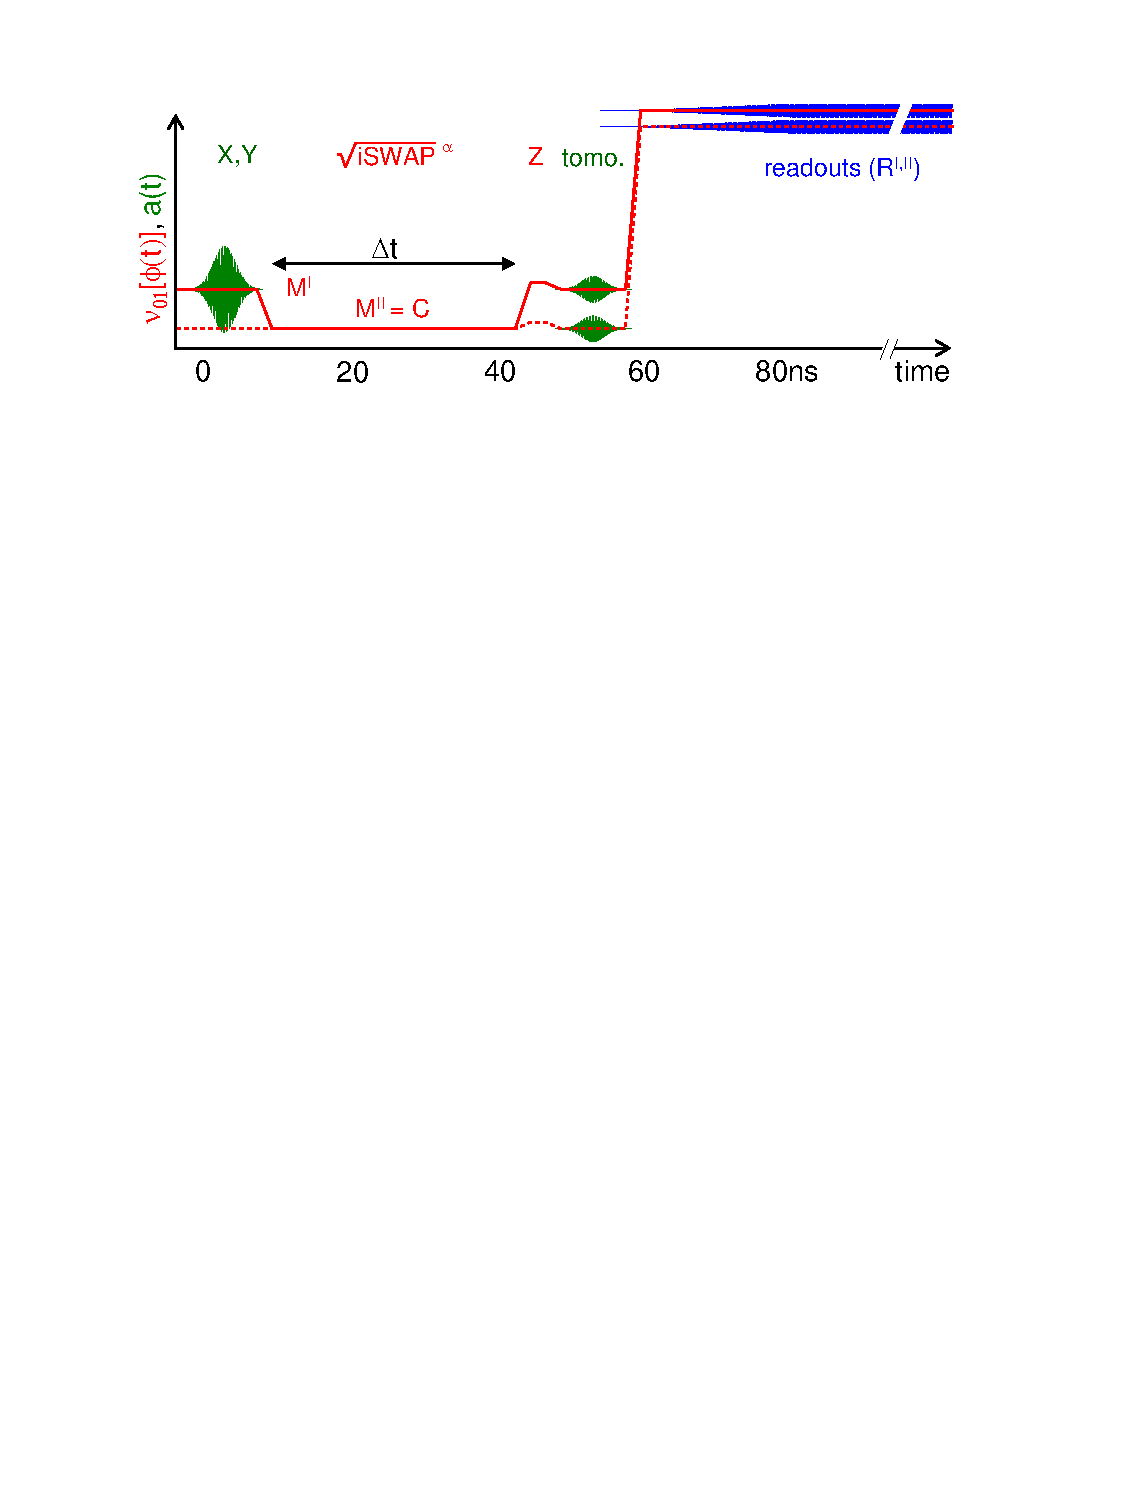
\includegraphics[width=0.8\textwidth]{./material/papers/iswap/figures/iswap_gate_pulse_sequence}
	\label{fig:ISwapPulseSequence}
	\caption{}
\end{figure}

\begin{figure}
  \flushright
	\includegraphics[width=1\textwidth]{"./data/ct5/2011_02_09 preparation of bell states/bell matrices"}
	\caption{Experimentially created $\ket{\psi_+}$ ($F = 0.91$) and $\ket{\psi_-}$ ($F=0.93$) states}
	\label{fig:BellStates}
\end{figure}

\subsection{Violation of the Bell Inequality}

\begin{figure}
	\centering
		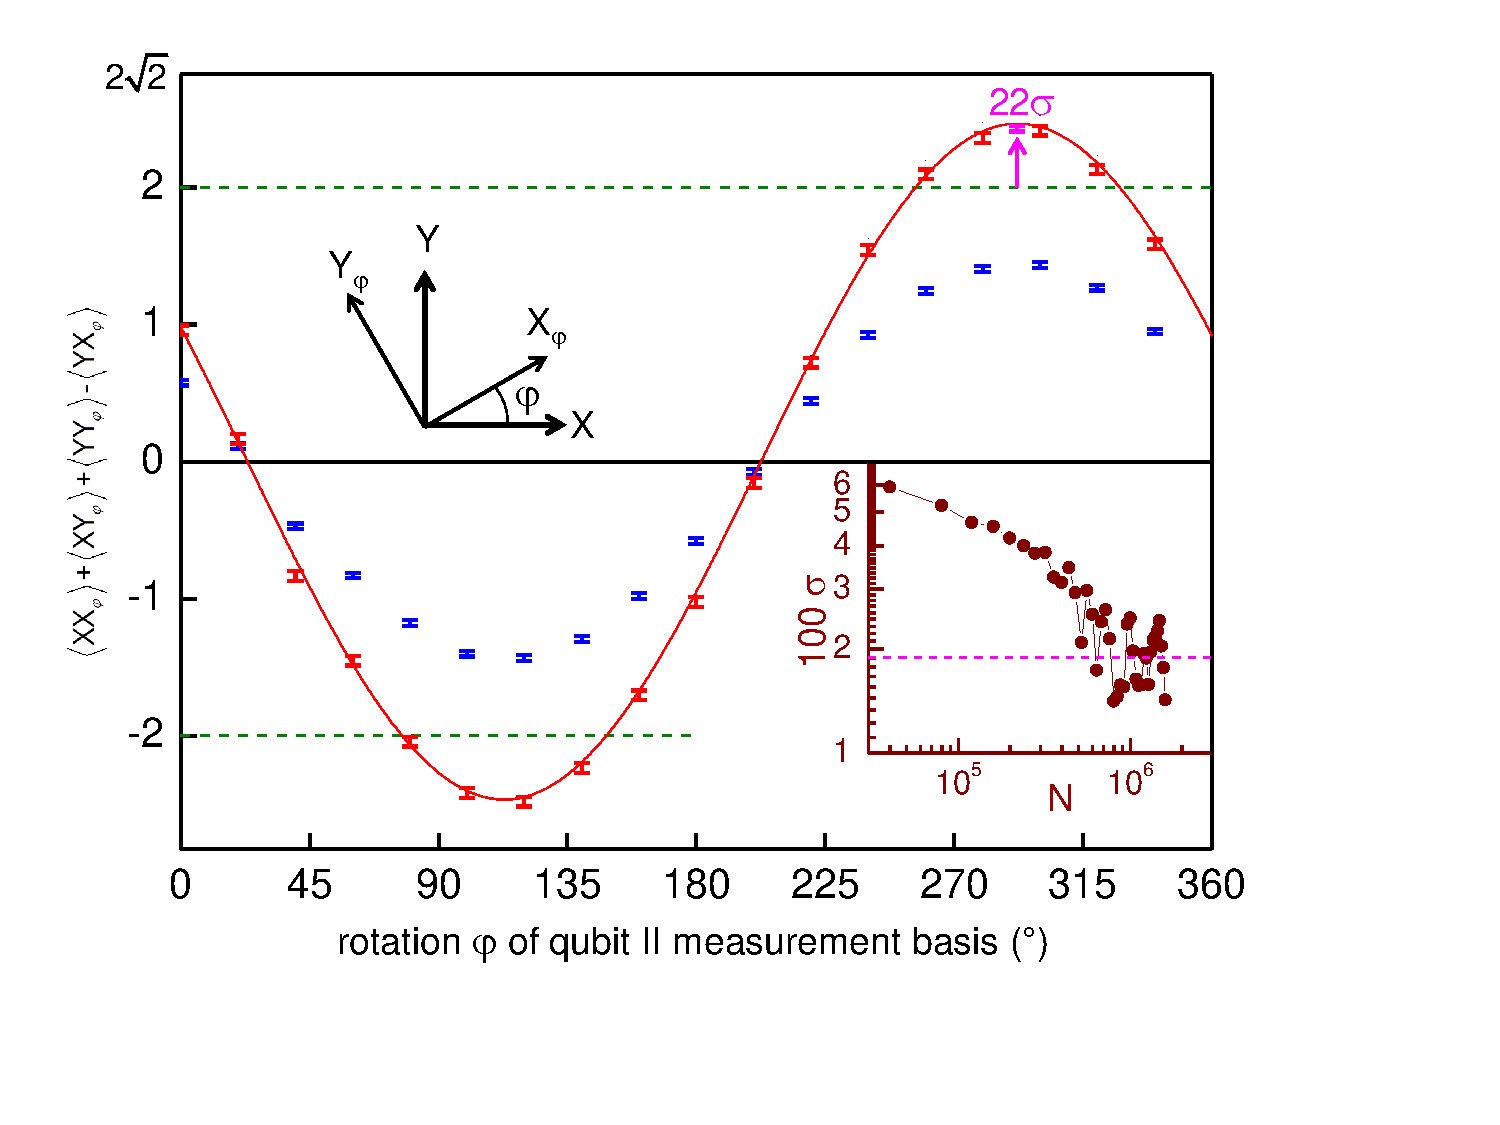
\includegraphics[width=0.8\textwidth]{./material/papers/iswap/figures/chsh}
	\label{fig:CHSH}
	\caption{}
\end{figure}


\subsection{Quantum State Tomography of Two-Qubit States}

Quantum state tomography is the procedure of experimentally determining an unknown quantum state\citep{michael_a._nielsen_quantum_2000}.

The density matrix of an n-qubit system can be written in general form as
\begin{eqnarray}
\rho & = & \sum\limits_{v_1,v_2\hdots v_n} \frac{c_{v_1,v_2\hdots v_n} \sigma_{v_1}\otimes \sigma_{v_2}\hdots \sigma_{v_n}}{2^n} \label{eq:state_tomography_state_representation} \\
c_{v_1,v_2\hdots v_n} & = & \mathrm{tr}\left(\sigma_{v_1}\otimes \sigma_{v_2}\hdots \otimes\sigma_{v_n} \; \rho \right)  \label{eq:state_tomography_coefficients}
\end{eqnarray}
where $v_i \in \left\{ X,Y,Z,I\right\}$ and $n$ gives the number of qubits in the system and where the $c_{v_1,v_2\hdots v_n}$ are real-valued coefficients that fully describe the given density matrix. To reconstruct the density matrix of an experimental quantum system in a well-prepared state it is therefore sufficient to measure the expectation values of these $n^2-1$ coefficients on an ensemble of identically prepared systems. However, statistical and systematic measurement errors can yield a set of coefficients that corresponds to a {\it non-physical} density matrix which violates either the positivity or unity-trace requirement. In the following paragraph we will therefore discuss a technique with which one can estimate the density matrix of a system in a more correct way.

\subsubsection{Maximum Likelihood Estimation of Quantum States}

A method which is often used in quantum state tomography is the so-called {\it maximum-likelihood} technique. Rather than directly calculating the density matrix of the system from the obtained expectation values $c_{v_1,v_2\hdots v_n}$, it calculates the joint probability of measuring a set $\{c_{X,X,\hdots,X},c_{Y,X,\hdots,X},\hdots,c_{I,I,\hdots,I}\}$ for a given estimate of the density matrix $\hat{\rho}$. By numerically or analytically maximizing this joint probability over the set of possible density matrices we obtain the density matrix which is most likely to have produced the set of measurement outcomes that we have observed.

The joint measurement operators $\Sigma_j = \sigma_{v_1}\otimes \sigma_{v_2}\hdots \otimes\sigma_{v_n}$ have the eigenvalues $\pm 1$ and can thus be written as 
\begin{equation}
\sigma_{v_1}\otimes \sigma_{v_2}\hdots \otimes\sigma_{v_n} = \ket{+_j}\bra{+_j}-\ket{-_j}\bra{-_j}
\end{equation}
where $\ket{-_j}$ and $\ket{-_j}$ are the eigenstates corresponding to the eigenvalues $\pm 1$ of $\Sigma_j$. The expectation value $\langle \Sigma_j \rangle$ can be estimated by the quantity
\begin{equation}
\widehat{\langle \Sigma_j \rangle}_\rho = \frac{1}{l}\sum\limits_{i = 1}^l M_i(\Sigma_j,\rho) \label{eq:tomography_measurement_estimator}
\end{equation}
 where $M_i(M,\rho)$ denotes the outcome of the $i$-th measurement of the operator $M$ on the state described by the density matrix $\rho$. This quantity is binomially distributed with the expectation value $E(\widehat{\langle \Sigma_j \rangle}_\rho) = \langle \Sigma_j \rangle_\rho$ and the variance $\sigma^2(\widehat{\langle \Sigma_j \rangle}_\rho) = 1/l \cdot (1-\langle \Sigma_j \rangle_\rho^2)$. For large sample sizes $l$, the binomial distribution can be well approximated by a normal distribution with the same expectation value and variance. The joint probability of obtaining a set of measurement values $\{s_1,\hdots,s_{n^2-1}\}$ for the set of operators $\{\widehat{\langle\Sigma_1 \rangle}_\rho,\hdots,\widehat{\langle\Sigma_{n^2-1} \rangle}_\rho\}$ is then given as
\begin{equation}
P\left(\widehat{\langle \Sigma_1 \rangle }_\rho = s_1;\hdots;\widehat{\langle \Sigma_{n^2-1} \rangle}_\rho =  s_{n^2-1}\right) = \prod\limits_{i = 1}^{n^2-1} \exp{\left(-\frac{l}{2}\frac{(s_i-\langle \Sigma_i \rangle_\rho)^2}{1-\langle \Sigma_i \rangle_\rho^2}\right)}
\end{equation}
By maximizing this probability (or the logarithm of it) we obtain an estimate of the density matrix $\rho$ of the quantum state. This technique also allows us to include further optimization parameters when calculating the joint probability. This is useful for modeling e.g. systematic errors of the measurement or preparation process, which can be described by modifying the operators contained in the probability sum. A common source of errors in our tomography measurements are errors in the microwave pulses used to drive the qubit. Since our measurement apparatus permits us only to measure the $\sigma_z$ operator of each qubit we have to perform $\pi/2$ rotations about the $Y$ or $-X$ axes of the Bloch sphere of each individual qubit in order to measure the values of the $\sigma_x$ and $\sigma_y$ operators, which we therefore replace with an effective measurement of each qubits $\sigma_z$ operator preceded by a rotation $R_{\nu_i}$ given as
\begin{eqnarray}
R_{X} & = & \exp{\left( -i \sigma_y \pi / 4\right)} \\
R_{Y} & = & \exp{\left( +i \sigma_x \pi / 4\right)} 
\end{eqnarray}
Phase and amplitude errors can be modeled as
\begin{eqnarray}
R_{X} & = & \exp{\left( -i \left[+\sigma_y\cos{\alpha}+\sigma_x\sin{\alpha} \right] \left[\pi / 4+\gamma\right]\right)} \\
R_{Y} & = & \exp{\left( +i \left[-\sigma_y\sin{\beta}+\sigma_x\cos{\beta}\right] \left[\pi / 4+\delta\right]\right)} 
\end{eqnarray}
Here, $\alpha$ and $\beta$ represent phase errors whereas $\gamma$ and $\delta$ represent amplitude errors in the drive pulses.

\section{Realizing a Two-Qubit Gate}

\begin{figure}
   \centering
	 \includegraphics[width=1.\textwidth]{"./data/ct5/film of swap/pauli_set_vs_time_with_simulation"}
	 \caption[test]{Measured Pauli operators $\sigma_i \otimes \sigma_j$ with $i,j \in \{X,Y,Z,I\}$ as a function of the interaction time. Shown are the 6 single-qubit operators as well as the 9 two-qubit correlation operators. The dashed line represents a master-equation simulation of the experiment.}
	 \label{fig:swap_pauli_set_vs_time_with_simulation}
\end{figure}

\subsection{Principle}

\begin{figure}[p]
	\centering
		\includegraphics[width=1.0\textwidth]{"./data/ct5/2011_04_21 - grover and tomo/good_data/process -matrices 1"}
	\label{fig:ProcessInputOutputMatrices1}
	\caption{The input-output density matrix of the quantum process tomography of the $\sqrt{i\mathrm{SWAP}}$ gate. Shown are the measured density matrices of 16 different input states and the corresponding output matrices with their state fidelities. The ideal matrices are overlaid in red.}
\end{figure}

\begin{figure}[p]
	\centering
		\includegraphics[width=1\textwidth]{"./data/ct5/2011_04_21 - grover and tomo/good_data/process -matrices 2"}
	\label{fig:ProcessInputOutputMatrices2}
	\caption{The input-output density matrix of the quantum process tomography of the $\sqrt{i\mathrm{SWAP}}$ gate. Shown are the measured density matrices of 16 different input states and the corresponding output matrices with their state fidelities. The ideal matrices are overlaid in red.}
\end{figure}

\subsection{Experimental Implementation}

\subsection{Quantum Process Tomography of the Gate}

\subsubsection{Introduction \& Principle}

\subsubsection{Implementation}

A quantum process can be described as a map $\mathcal{E} : \rho_\mathcal{H} \to \rho_\mathcal{H}$ that maps a density matrix $\rho$ defined in a Hilbert space $Q_1$ to another density matrix $\mathcal{E}(\rho)$ defined in a target Hilbert space $Q_2$ and fulfilling three axiomatic properties \cite{michael_a._nielsen_quantum_2000,haroche_exploring_2006}:

\begin{axiom}
$\mathrm{tr}\left[\mathcal{E}(\rho)\right]$ is the probability that the process represented by $\mathcal{E}$ occurs, when $\rho$ is the initial state.
\end{axiom}

\begin{axiom}
$\mathcal{E}$ is a {\it convex-linear map} on the set of density matrices, that is, for probabilities $\left\{p_i\right\}$,

  \begin{equation}
	  \mathcal{E}\left(\sum\limits_i p_i \rho_i\right) = \sum\limits_i p_i \mathcal{E}(\rho_i)
	\end{equation}
\end{axiom}

\begin{axiom}
$\mathcal{E}$ is a {\it completely-positive} map. That is, if $\mathcal{E}$  maps density operators of system $Q_1$ to density operators of system $Q_2$, then $\mathcal{E}(A)$ must be positive for any positive operator $A$. Furthermore, if we introduce an extra system $R$ of arbitrary dimensionality, it must be true that $(\mathcal{I}\otimes \mathcal{E})(A)$ is positive for any positive operator $A$ on the combined system $RQ_1$, where $\mathcal{I}$ denotes the identity map on system $R$.
\end{axiom}
As shown in \cite{michael_a._nielsen_quantum_2000}, any quantum process fulfilling these criteria can be written in the form

\begin{equation}
  \mathcal{E}(\rho) = \sum\limits_i E_i \rho E_i^\dagger \label{eq:process_operator_sum_representation}
\end{equation}
for some set of operators $\{ E_i \}$ which map the input Hilbert space to the output Hilbert space, and $\sum_i E_i^\dagger E_i \le I$.

Now, if we express the operators $E_i$ in a different operator basis $\tilde{E}_j$ such that $E_i = \sum_j a_{ij} \tilde{E}_{j}$ and insert into eq. (\ref{eq:process_operator_sum_representation}), we obtain

\begin{eqnarray}
 \mathcal{E}(\rho) & = & \sum\limits_i \sum\limits_j a_{ij} \tilde{E}_j \;\rho\; \sum\limits_k a_{ik}^* \tilde{E}_k^\dagger \\
& = & \sum\limits_{j,k}\tilde{E}_j \; \rho \; \tilde{E}_k^\dagger \sum\limits_i a_{ij} a_{ik}^* \\
& = & \sum\limits_{j,k}\tilde{E}_j \; \rho \; \tilde{E}_k^\dagger \; \chi_{jk} \label{eq:process_chi_representation}
\end{eqnarray}
where we defined $\chi_{jk} = \sum\limits_i a_{ij} a_{ik}^*$. This is the so-called $\chi$-matrix representation of the quantum process. Here, all the information on the process is contained in the $\chi$ matrix, which controls the action of the process-independent operators $\tilde{E}_i$ on the initial density matrix $\rho$.

Now, the goal of {\it quantum process tomography} is to obtain the coefficients of the $\chi$-matrix -- or any other complete representation of the process -- from a set of experimentally measured density matrices $\rho$ and $\mathcal{E}(\rho)$.

To achieve this, several techniques have been developed. The technique used in this work is the so-called {\it standard quantum process tomography (SQPT)}. This technique proceeds as follows:

\begin{enumerate}
\item Choose a set of operators $E_i$ that forms a full basis of $\mathcal{M}: Q_1 \to Q_2$. For n-qubit process tomography we usually choose $E_{i_1,i_2 \hdots i_n} = \sigma_{i_1}\otimes \sigma_{i_2}\hdots\otimes\sigma_{i_n}$, where $\sigma_i$ are the single-qubit Pauli operators and $i\in\{I,X,Y,Z\}$. 
\item Choose a set of pure quantum states $\ket{\phi_i}$ such that $\ket{\phi_i}\bra{\phi_i}$ span the whole space of input density matrices $\rho$. Usually, for a n-qubit system we choose $\phi = \{\ket{0},\ket{1},(\ket{0}+\ket{1})/\sqrt{2},(\ket{0}+i\ket{1})/\sqrt{2}\}^{\otimes n}$, where $^{\otimes n}$ denotes the n-dimensional Kronecker product of all possible permutations.
\item For each of the $\ket{\phi_i}$, determine $\mathcal{E}(\ket{\phi_i}\bra{\phi_i})$ by quantum state tomography. Usually we also determine $\ket{\phi_i}\bra{\phi_i}$ experimentally since the preparation of this state already entails small preparation errors that should be taken into account when performing quantum process tomography. 
\end{enumerate}

After having obtained the $\rho_i$ and $\mathcal{E}(\rho_i)$ one obtains the $\chi$-matrix by writing $\mathcal{E}(\rho_i) = \sum_j \lambda_{ij} \tilde{\rho}_j$, with some arbitrary basis $\tilde{\rho}_j$ and
letting $\tilde{E}_m \tilde{\rho}_j \tilde{E}_n^\dagger = \sum_k \beta_{jk}^{mn}\tilde{\rho}_k$. We can then insert into eq. (\ref{eq:process_chi_representation}) and obtain
\begin{eqnarray}
\sum\limits_k \lambda_{ik} \tilde{\rho}_k & = & \sum\limits_{m,n} \chi_{mn} \sum\limits_k \beta_{ik}^{mn} \tilde{\rho}_k  
\end{eqnarray}
This directly yields $\lambda_{ik} = \sum_{m,n}\beta_{ik}^{mn}\; \chi_{mn}$, which, by linear inversion,  gives $\chi$.

\subsubsection{The Kraus Representation of the Quantum Process}

Besides the $\chi$-matrix representation, there is another useful way of expressing a quantum map, the so called {\it Kraus representation}, which is given as

\begin{equation}
 \mathcal{E}(\rho) = \sum\limits_i M_i \; \rho \; M_i^\dagger \label{eq:process_kraus_representation}
\end{equation}

It can be shown \citep{haroche_exploring_2006} that this sum contains at most $N$ elements, where $N$ is the dimension of the Hilbert space of the density matrix $\rho$. We can go from the $\chi$ representation to the Kraus representation by changing the basis $\tilde{E}_i$ such that

\begin{equation}
	\tilde{E}_i = \sum\limits_l a_{il}\; \breve{E}_l
\end{equation}

which, for eq. (\ref{eq:process_chi_representation}), yields

\begin{eqnarray}
 \mathcal{E}(\rho) & = & \sum\limits_{j,k} \sum\limits_l a_{jl} \breve{E}_l \; \rho \sum\limits_m a_{km}^* \breve{E}_m^\dagger \; \chi_{jk} \\
 & = & \sum\limits_{l,m}  \breve{E}_l \; \rho \; \breve{E}_m^\dagger \; \sum\limits_{j,k} a_{jl} a_{km}^* \chi_{jk} \label{eq:process_chi_transformed}
\end{eqnarray}

The last sum on the right side of eq. (\ref{eq:process_chi_transformed}) corresponds to a change of coordinates of the matrix $\chi$. Now, we can pick the $a$ such that $\chi$ is diagonal in the new basis $\breve{E}$ and obtain

\begin{eqnarray}
 \mathcal{E}(\rho) & = &  \sum\limits_{l} \lambda_l \breve{E}_l \; \rho \; \breve{E}_l^\dagger \\
& = &  \sum\limits_{l} M_l \; \rho \; M_l^\dagger
\end{eqnarray}
with $\lambda_l$ being the $l$-th eigenvalue of the $\chi$ matrix with the eigen-operator $\breve{E}_l$ and $M_{l} = \sqrt{\lambda_l} \breve{E}_l$.

\subsection{Gate Fidelity}

\subsection{Gate Error Analysis}

%-Discuss the realization of a 2 qubit gate:
%  -Principle
%  -Implementation & Pulse Sequency
%  -Characterization through Quantum Process Tomography:
%     -Principles: State tomography, Pauli set, process tomography
%     -Discuss alternative representations of the process information:
%        -Chi matrix, Choi matrix, S, log S, Kraus operator representation
%  		-Errors: Discuss simulations, error models and possible reasons for discrepancies

\begin{figure}
	\centering
		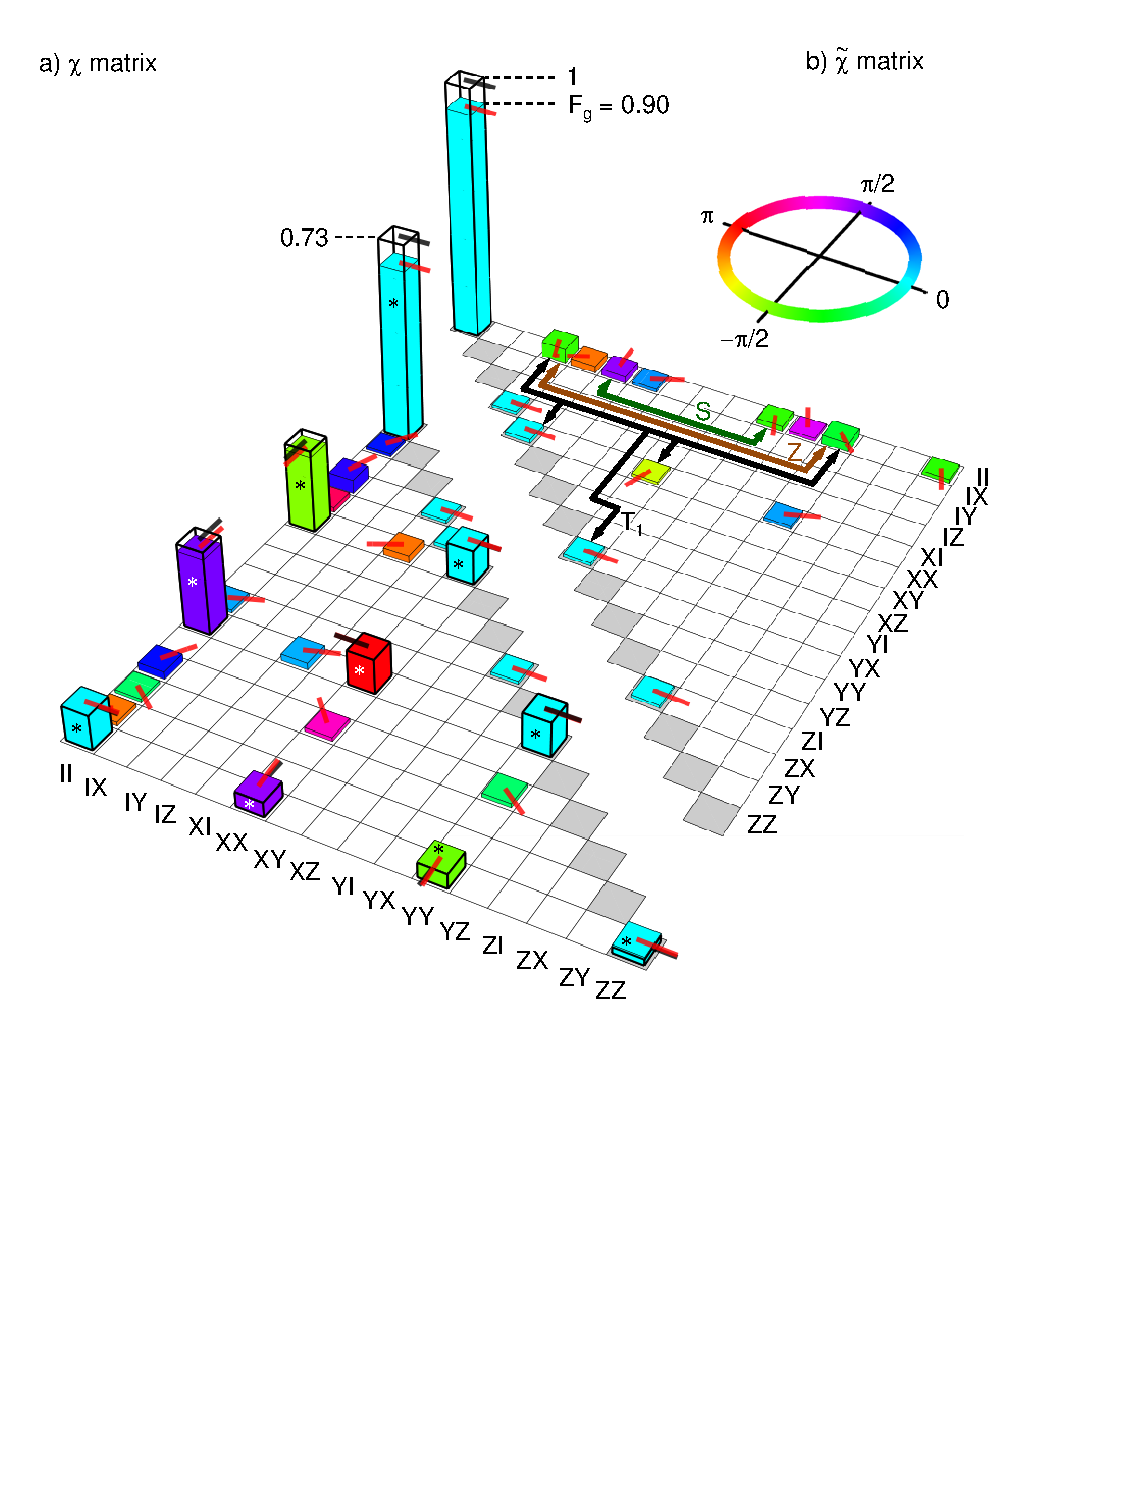
\includegraphics[width=1.\textwidth]{./material/papers/iswap/figures/chi_matrix_and_error_process}
	\label{fig:GateChiMatrixAndErrorProcess}
	\caption{}
\end{figure}


\chapter{Running the Grover Search Algorithm}

%Motivate this experiment:
% -Benchmark for superconducting quantum computers
% -Speed-up for searching in an unsorted database

\section{Introduction \& Motivation}

The original algorithm by as given by \cite{Grover_Quantum_1997} is given as follows

\begin{enumerate}
 \item Start with the qubit register in the state $\ket{\psi} = \ket{000\hdots 0}$
 \item Apply the Hadamard operation to the qubit register, producing the equally superposed state $$\ket{\psi} = \frac{1}{\sqrt{n}}\sum\limits_i^n \ket{i}$$.
 \item Repeat the following sequence $\begin{mathcal}O\end{mathcal}(\sqrt{n})$ times:
 \subitem Apply the oracle operator $\ket{i}\to (-1)^{\delta_i^j}\ket{i}$ to the state $\ket{\psi}$, where $\ket{j}$ is the state marked by the oracle.
 \subitem Apply the diffusion operator $\ket{i} \to -\ket{i}+\frac{2}{n}\sum\limits_i^n\ket{j}$ to the state $\ket{\psi}$.
	\item Measure the state of the quantum register
\end{enumerate}

The seemingly elusive algorithm can be derived in a very clear way from Schrödinger's equation, as shown in the seminal paper by \cite{grover_schrodingers_2001}. Since the derivation given in this paper sheds some interesting light on the nature of the quantum search algorithm we will discuss it here. The derivation begins by considering a quantum system governed by Schrödinger's equation, which can be written as (omitting all physical constants for the sake of clarity)

\begin{equation}
-i\frac{\delta}{\delta t}\psi(x,t) = \frac{\delta^2}{\delta x^2}\psi(x,t)-V(x)\psi(x,t) \label{eq:grover_derivation}
\end{equation}

Here $\psi(x,t)$ describes the wave-function and $V$ is a time-indepenent potential. Let us assume that the potential $V(x)$ is shaped as in fig. \ref{fig:grover_derivation}a, i.e. possessing a local minimum of energy. When one initializes the system to a state $\psi_0(x,t_0)$ and lets it evolve for a given time, the resulting state $\psi(x,t)$ will have a tendency to have a high probability density in the local minimum of the potential, thus ``falling'' into the potential minimum much like a classical system would.

It is thus interesting to ask if one could encode the solution to some hard problem as a point of minimum energy $x_0$ of a potential $V(x)$ and design an algorithm that would take an initial state $\psi_0(x,t_0)$ and let it evolve into a state that has a high probability around $x_0$. Most problems in classical computer science involve functions operating on binary numbers of fixed length, so to encode these numbers we can discretize our wavefunction $\psi(x,t)$ using a regular grid of points $x_i$ with a spacing $dx$, as shown in fig. \ref{fig:grover_derivation}b. When we discretize the time evolution of eq. \ref{eq:grover_derivation} in steps $dt$ as well and define $\epsilon = dt/dx^2$, we obtain a new equation of the form

\begin{equation}
-\frac{\psi_i^{t+dt}-\psi_x^{t}}{dt} = \frac{\psi_{i+1}^t+\psi_{i-1}^t-2\psi_x^t}{dx^2} -V(x_i)\psi_i^t
\end{equation}

where we have written $\psi(x_i,t)=\psi_i^t$. This equation can be written in matrix form as

\begin{equation}
\vec{\psi}^{t+dt} = S^t  \cdot \vec{\psi}^t
\end{equation}

with $S$ being a state transition matrix of the form

\begin{equation}
S = \left(
	\begin{array}{ccccc}
		1-2i\epsilon-iV(x_1)dt & i\epsilon & 0 & \hdots &  i\epsilon \\
		i \epsilon & 1-2i\epsilon -iV(x_2)dt & i\epsilon & \hdots & 0 \\
		0 & i\epsilon & \ddots & & \vdots \\
		\vdots & & & \ddots  & \vdots \\
		i \epsilon & 0 & \hdots & i\epsilon & 1 - 2i\epsilon -iV(x_n)dt
	\end{array}
 \right) \label{eq:grover_iteration_matrix}
\end{equation}

where we have used cyclic boundary conditions and defined $\epsilon = dt/dx^2$. To calculate the wavefunction at a finite evolution time we make use the Lie-Trotter formula

\begin{equation}
\exp{\left(A+B\right)} = \lim\limits_{N\to\infty}\left(\exp{\left(A/N\right)}\exp{\left(B/N\right)}\right)^N
\end{equation}

to write $\exp{\left(S\right)} \approx D\cdot R$ with 

\begin{eqnarray}
D & = & \left( 
		\begin{array}{cccccc}
		1-2i \epsilon & i\epsilon & 0 & 0 & \hdots & i\epsilon \\
		i \epsilon & 1 - 2i \epsilon & i \epsilon & 0 & \hdots & 0 \\
		\hdots & \ddots & & & & \vdots \\
		i \epsilon & 0 & 0 &  \hdots & i\epsilon & 1-2i \epsilon \\
		\end{array}
	\right)
\end{eqnarray}
and 
\begin{eqnarray}
R & = & \left( \begin{array}{ccccc}
	e^{-i V(x_1) dt} & 0 & \hdots & 0 \\
	0 & e^{-i V (x_2) dt} & \hdots & 0 \\
	0 & \hdots & & 0 & e^{-i V (x_n) dt} \\
	\end{array}
	\right)
\end{eqnarray}

This approximation is correct to $\begin{mathcal}O\end{mathcal}(\epsilon)$ up to an unrelevant renormalization factor. The technique of splitting up the full evolution operator into a product of two or more non-commuting evolution operators that are applied successively is widely used in digital quantum simulation \citep{lloyd_universal_1996,lanyon_universal_2011}. We can now repeatedly apply the matrix product $D\cdot R$ to the waveunction to obtain its state after a given finite time $\Delta t$ by writing

\begin{equation}
\vec{\psi}^{t+\Delta t} = \left(\prod\limits_{i = 1}^{\Delta t/dt} D\cdot R\right)\cdot \vec{\psi}^{t}
\end{equation}

Using this approach, the evolution of the wavefunction is governed by two processes: The interaction of the wavefunction with the potential $V$ and a diffusion process which mixes different spatial parts of the wavefunction. The operator $D$ resembles a Markov diffusion process since each row and column of the matrix sums up to unity, whereas $R$ changes the phase of each element of the wavefunction in accordance with the local potential seen by it. If we apply $R$ to an initial state of the form $\psi_i = 1$ (we omit the normalization factor for clarity) and assume that $V_i = 0$ for $i \ne j$ and $V_j dt = \phi$, the element $\psi_j$ will get turned according to $\psi_j \to \psi_j \exp{\left(i\phi\right)}$.. Applying the operator $D$ to the resulting state will transform $\psi_j$ according to $\psi_j \to \psi_j(i+2\epsilon(1+i))$ with a corresponding amplitude $\sqrt{1+4\epsilon+\begin{mathcal}O\end{mathcal}(\epsilon^2)}$ and the adjacent states $\psi_{j\pm 1}$ according to $\psi_{j\pm 1} \to \psi_{j\pm 1}(1-\epsilon(1+i))$ with an amplitude $\sqrt{1-2\epsilon +\begin{mathcal}O\end{mathcal}(\epsilon^2)}$. Hence there is a transfer of amplitude between the state whose phase has been turned and its neighboring states. If we could reset the phases of the components of $\vec{\psi}$ afterwards, we would be able to iterate the application of $D\cdot R$ until all of the amplitude would have been transferred to the $\psi_j$. This, in essence, is what the Grover algorithm accomplishes by replacing the matrix $D$ with an unitary matrix 

\begin{equation}
D' = \left( \begin{array}{ccccc}
	-1+2/n & 2/n & 2/n & \hdots & 2/n \\
	2/n & -1 + 2/n & 2/n & \hdots & 2/n \\
	\vdots & & \ddots & 2/n & \vdots \\
	2/n & 2/n & 2/n & \hdots & -1 + 2/n \\ 
	\end{array} \right) \label{eq:GroverDiffusionOperator}
\end{equation}

and $R$ with an unitary matrix 

\begin{eqnarray}
R' & = & \mathrm{I}^{n\otimes n}-2\ket{j}\bra{j} \label{eq:GroverOracleFunction}
\end{eqnarray}

where $j$ is the index of the searched basis state. When applying $D\cdot R$ to a fully superposed state $\vec{\psi}$, a maximum amount of amplitude will be transferred to the basis state $\psi_j$ marked by $R$. By repeating the $D\cdot R$ sequence $\begin{mathcal}O\end{mathcal}(\sqrt{n})$ times we can transfer all the amplitude into this basis state, therefore solving the search problem.

\subsection{Ancilla-based Implementation of the Algorithm}

\begin{figure}[ht!]
	\centering
		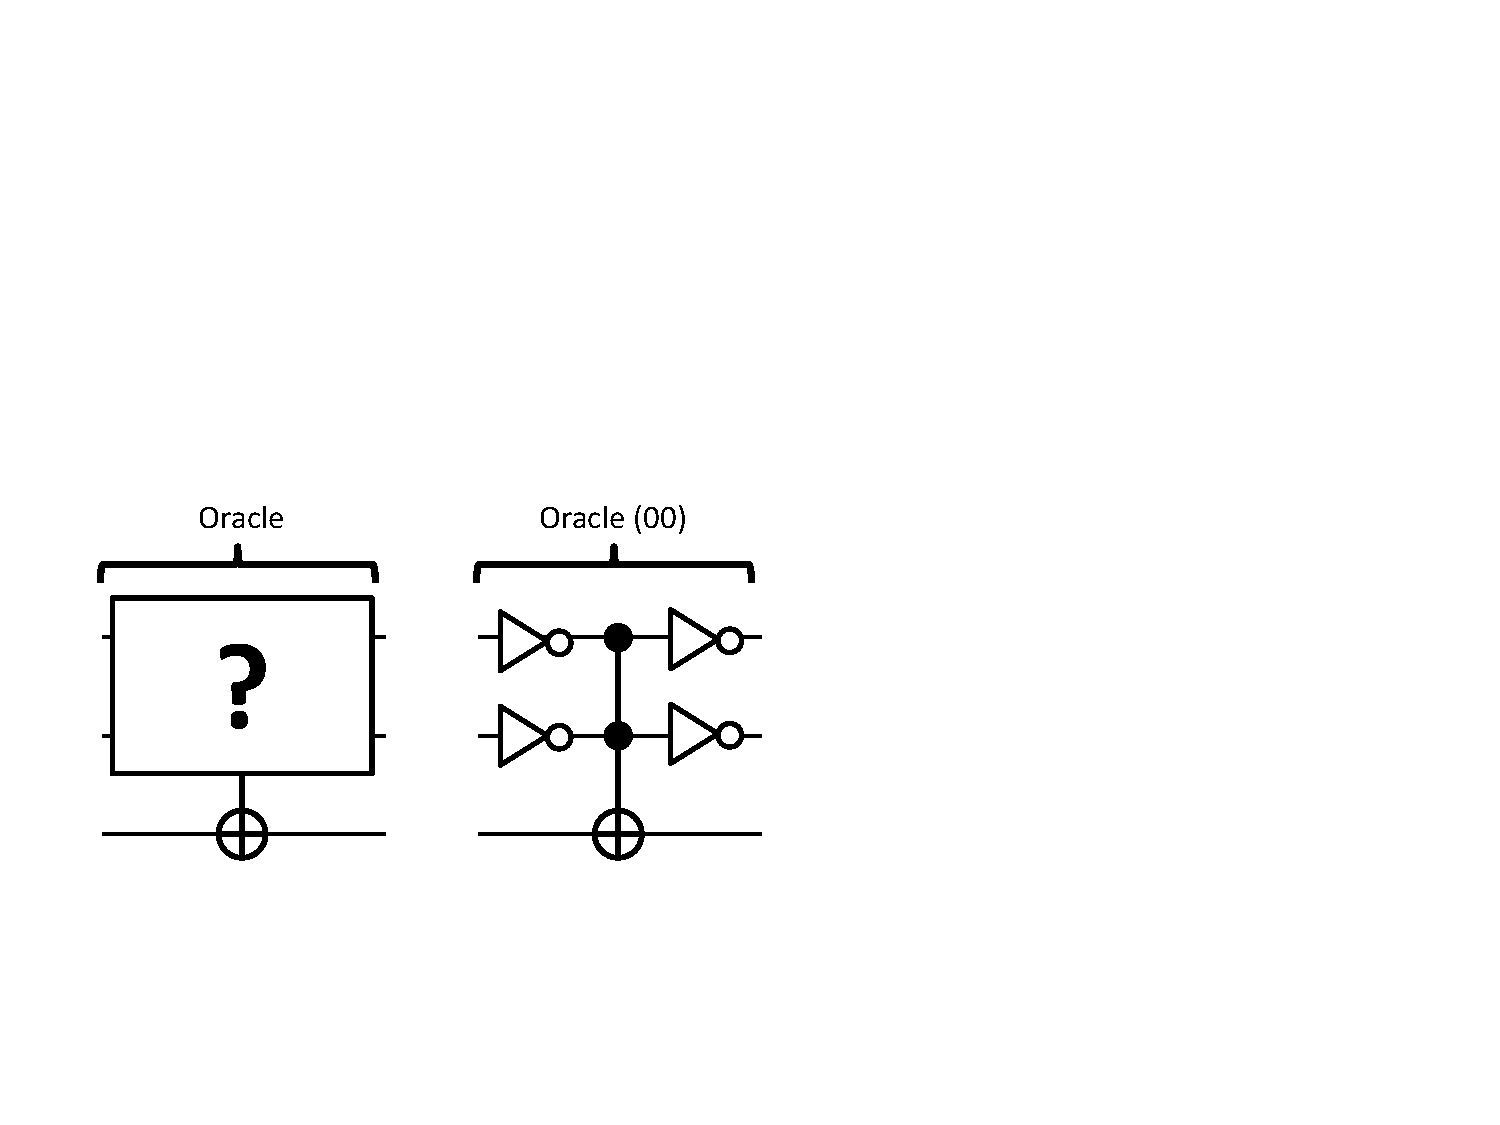
\includegraphics[width=1\textwidth]{./material/papers/grover/different_oracle_implementations}
	\caption[Implementations of the four possible Oracle functions used in the Grover search algorithm, using only reversible gate operations]{Implementations of the four possible Oracle functions used in the Grover search algorithm, using only reversible gate operations.}
	\label{fig:GroverOracleImplementations}
\end{figure}

It is also possible to define a version of the Grover algorithm where the Oracle function does not encode the marked state directly in the input qubit register but where it uses an ancialla qubit to store the information on the marked state. Possible implementations of such ancilla-based Quantum oracle functions for the two-qubit case are shown in fig. \ref{fig:GroverOracleImplementations}. There, a two-qubit Tofolli gate in combination with several single-qubit NOT gates (which can be easily implemented as single-qubit $X_{\pi}$ rotations) is used to flip the state of an ancilla-qubit conditionally on the input state of the gate. This gate is fully reversible and operates on product- as well as superposition states. Representing the quantum Oracle in this form is quite useful since it will allow us to compare the Grover algorithm with a classical search algorithm implemented using reversible gates. This will in turn allow us to compare the fidelity and success probability with that of a classical algorithm and thereby quantify the quantum speed-up achieved with our system. 

\begin{figure}[ht!]
	\centering
		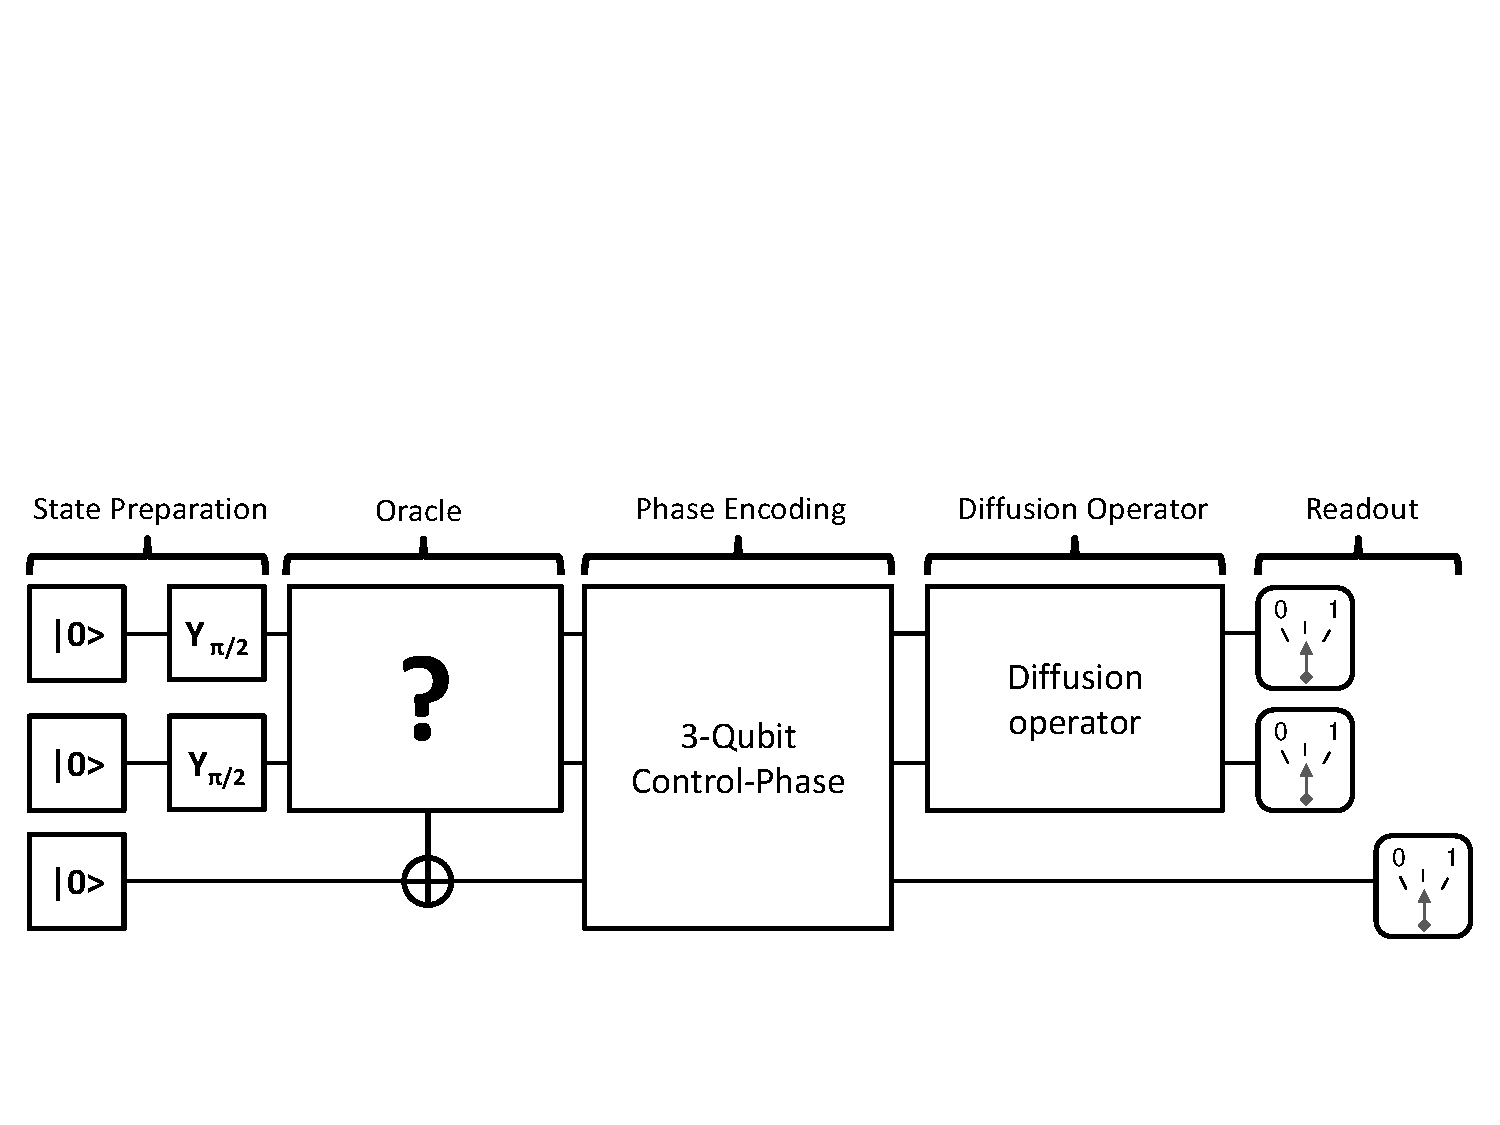
\includegraphics[width=1\textwidth]{./material/papers/grover/quantum_algorithm_full}
	\caption[Full version of an implementation of the two-qubit Grover search algorithm]{A full version of an implementation of the two-qubit Grover search algorithm. This algorithm works on a two-qubit input state and flips the state of a control qubit for one of the four possible input states in accordance to an unknown Oracle function. It then applies a 3-qubit control-phase operation of that maps $\ket{xx1}\to -\ket{xx1}$, $\ket{xx0}\to\ket{xx0}$ to encode the state of the control qubit directly in the two input qubits and then uses a diffusion operator to determine the state which has been marked by the Oracle function.}
	\label{fig:GroverAlgorithmFullSchematic}
\end{figure}

\smallskip

Fig. \ref{fig:GroverAlgorithmFullSchematic} shows an implementation of the two-qubit Grover algorithm which uses the ancilla-based Oracle function. This algorithm proceeds almost identically as the compiled version which we will present in the next section, with the difference that it uses a 3-qubit control-not gate $C$ of the form

\begin{equation}
C = \mathrm{I}^{n\otimes n}-2\sum\limits_{ij} \ket{ij1}\bra{ij1}
\end{equation}

which flips the sign of all states where the ancilla qubit is in state $\ket{1}$ and hence converts the ancilla-based quantum Oracle into the phase-encoded version that was outlined before. Here, the ancilla qubit must not be read out before the two input qubits since otherwise the algorithm will fail. One can verify that the Oracle function has really marked one of the basis states by reading out the value of the ancilla qubit after having read out the other qubits and checking for a value of $\ket{1}$.

\section{Experimental Implementation}

\begin{figure}[ht!]
	\centering
		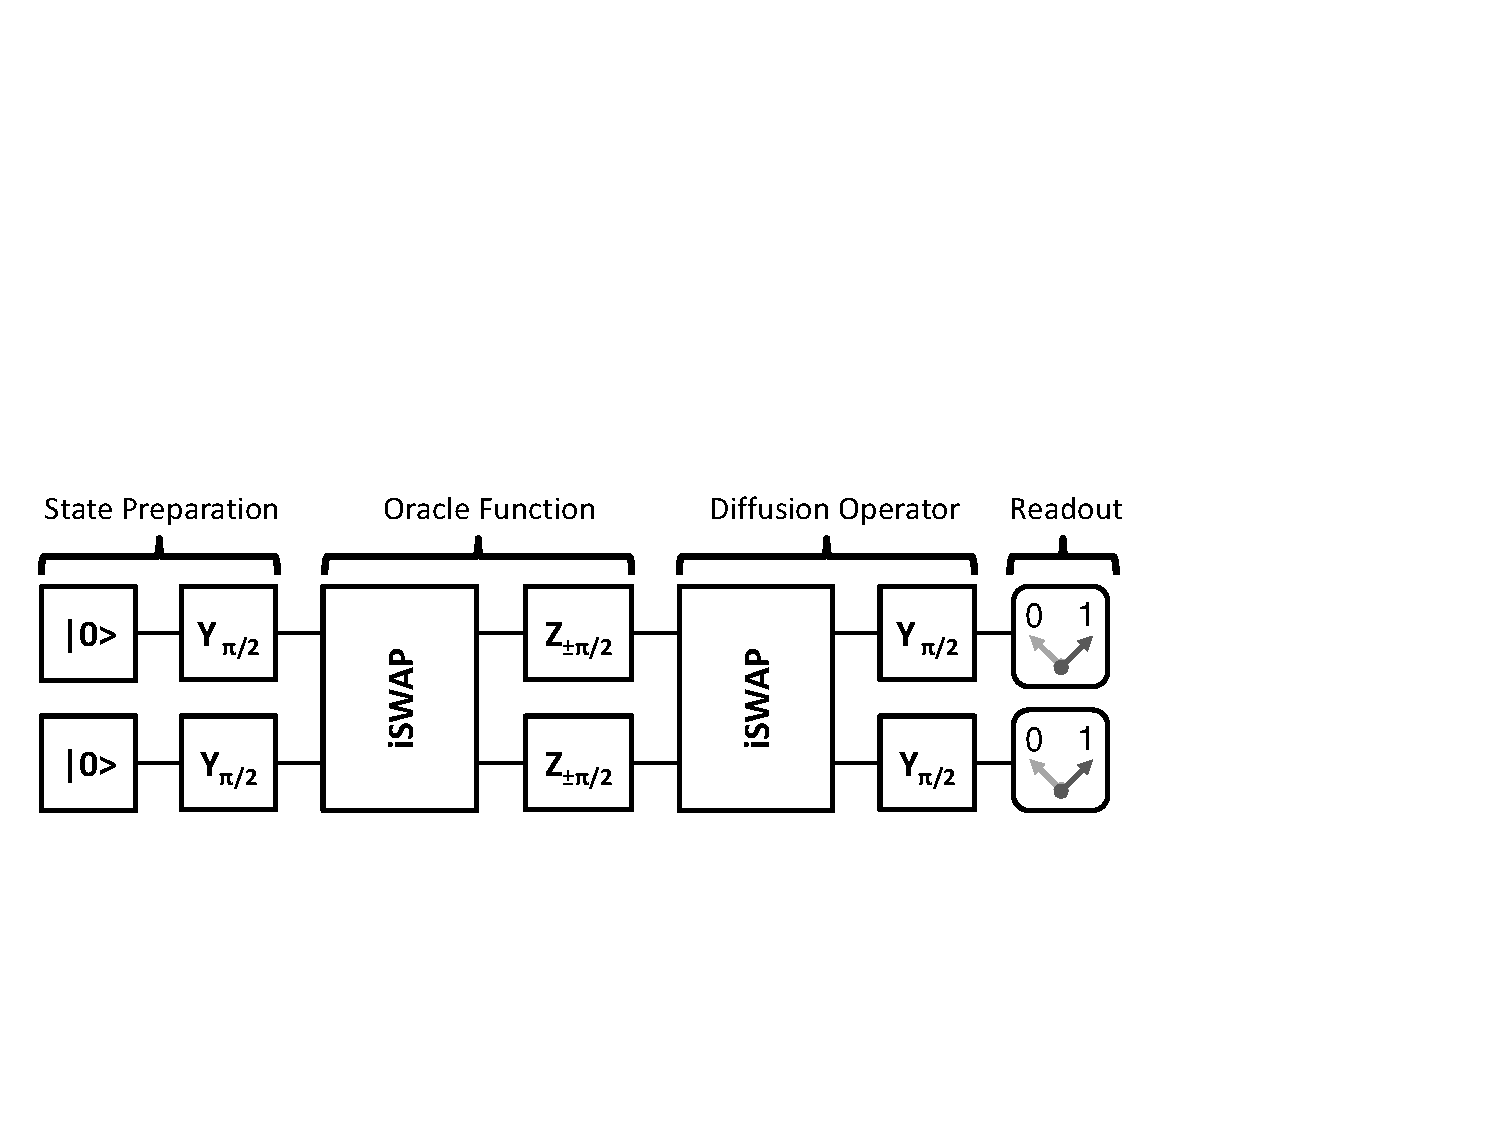
\includegraphics[width=0.8\textwidth]{./material/papers/grover/grover_algorithm}
	\caption[Schematic of our implementation of the Grover search algorithm]{Schematic of our implementation of the Grover search algorithm. The algorithm consists in generating a fully superposed input state, applying the Oracle function to it and analyzing the resulting state by applying the Diffusion transform to it and reading out the value of the qubit register afterwards.}
	\label{fig:GroverAlgorithmSchematic}
\end{figure}

In this work we implement a compiled version of the two-qubit Grover algorithm. The gate sequence of the algorithm is shown in fig. \ref{fig:GroverAlgorithmSchematic} and consists in two $i\mathrm{SWAP}$ gates and six single-qubit gates applied to an initial state $\ket{00}$. The first $i\mathrm{SWAP}$ gate together with the two single-qubit $Z_{\pm \pi}$ rotations implements the Oracle function $f(x)$ as given in eq. (\ref{eq:GroverOracleFunction}), where the signs of the rotation operations determines the state which is marked and can be either $\ket{00}$ (corresponding to a $Z^1_{-\pi/2}\cdot Z^2_{-\pi/2}$ rotation), $\ket{01}$ ($Z^1_{-\pi/2}\cdot Z^2_{\pi/2}$), $\ket{10}$ ($Z^1_{\pi/2}\cdot Z^2_{-\pi/2}$) or $\ket{11}$ ($Z^1_{\pi/2}\cdot Z^2_{\pi/2}$). The second $i\mathrm{SWAP}$ operation together with the following $X^1_{\pi/2}\cdot X^2_{\pi/2}$ operation implements the difussion operator as given by eq (\ref{eq:GroverDiffusionOperator}). The final step of the algorithm consists in reading out the two-qubit register.

\subsection{Pulse Sequence}

\begin{figure}[htb!]
	\centering
		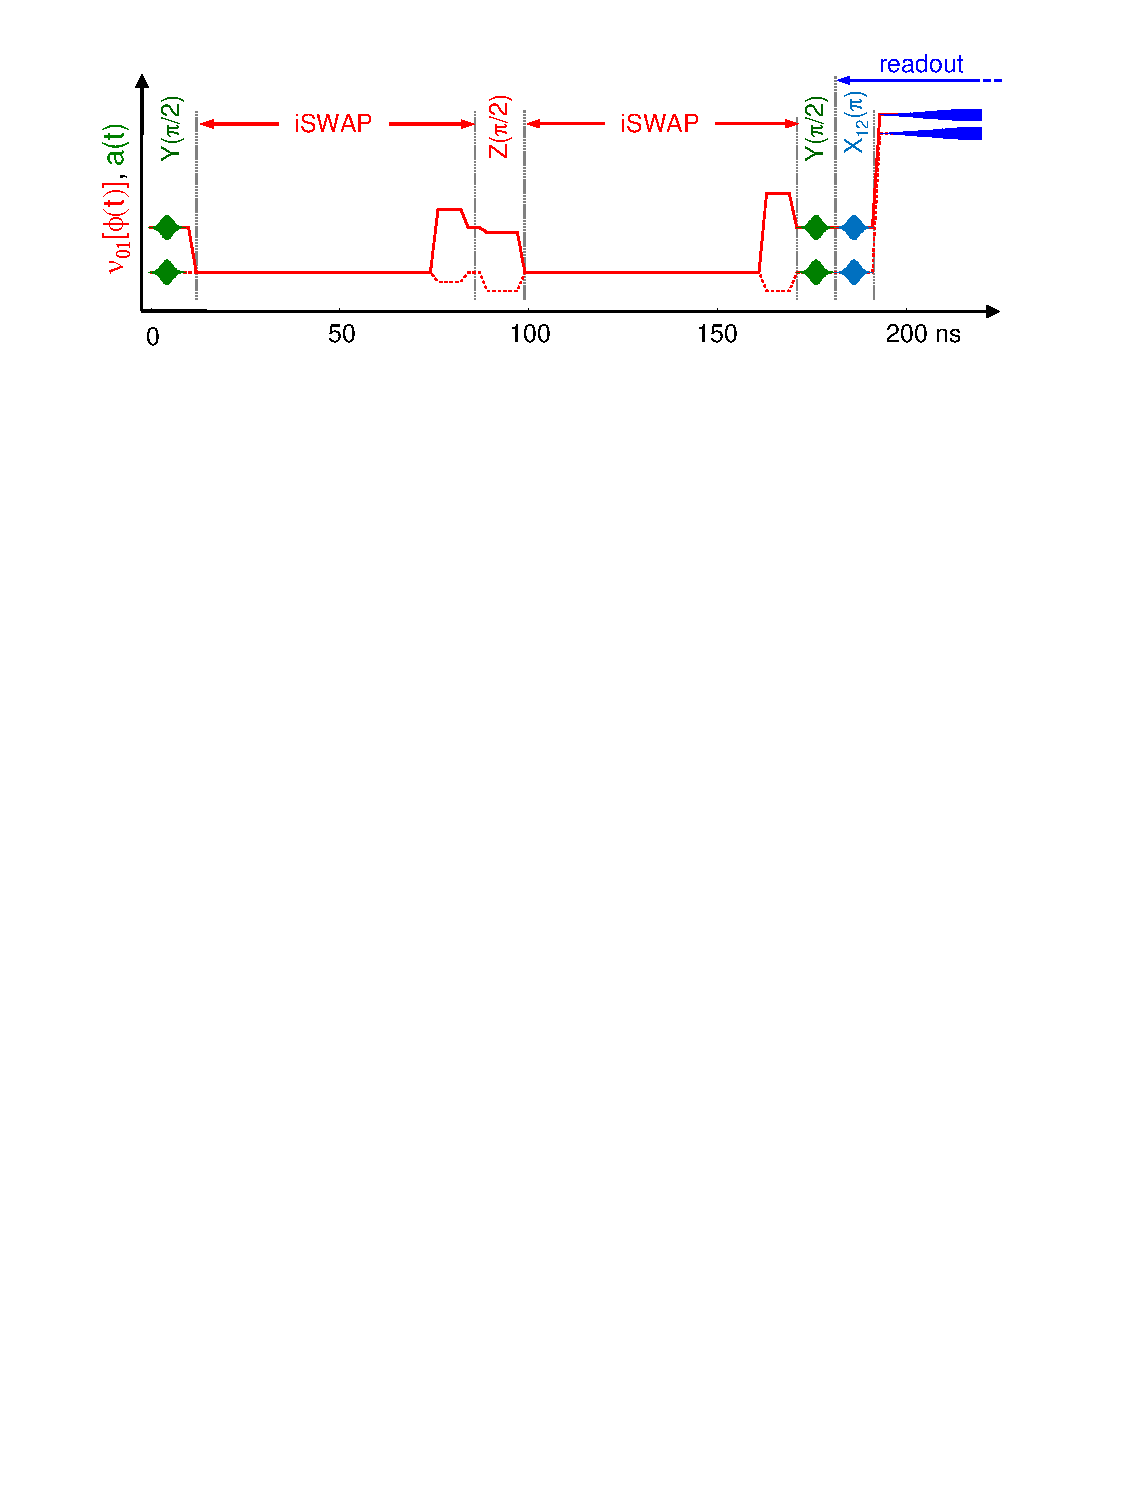
\includegraphics[width=1.\textwidth]{./material/papers/grover/figures/grover_algorithm_pulse_sequence}
	\label{fig:Grover3}
	\caption[Pulse sequence used for implementing Grovers search algorithm]{The pulse sequence used in realizing Grover's quantum search algorithm. First, a $Y_{\pi/2}$ pulse is applied to each qubit to produce the fully superposed state $1/2(\ket{00}+\ket{01}+\ket{10}+\ket{11})$. Then, an $i\mathrm{SWAP}$ gate is applied, followed by a $Z_{\pm \pi /2}$ gate on each qubit, which corrsponds to the application of the oracle function. The resulting state is then analyzed using another $i\mathrm{SWAP}$ gate and two $Y_{\pi/2}$ gates to extract the state which has been marked by the oracle function. Optionally, a $Y^{12}_{\pi}$ pulse is used on each qubit to increase the readout fidelity.}
\end{figure}


%\begin{landscape}

\begin{figure}
	\centering
		\rotatebox{90}{\includegraphics[width=1.2\textwidth]{"./data/ct5/2011_04_21 - grover and tomo/good_data/grover algorithm - single run results"}}
	\caption[Quantum state tomographies at different steps during the Grover search algorithm and single-run outcome probabilities]{Quantum state tomographies at different steps of the Grover search algorithm and single-run outcome probabilities. The density matrices show the experimentally measured states in color and the theoretical states in black. For each state, the trace fidelity $F_{tr}(\rho_A,\rho_B) = \mathrm{Tr}\{\rho_A\cdot\rho_B\}$ is shown above the density matrix.}
	\label{fig:GroverAlgorithmExperimentalResults}
\end{figure}

%\end{landscape}

\section{Algorithm Fidelity}

Likewise we can define the average fidelity of the algorithm in a single run, which corresponds to the averaged success probabilities measured for all four Oracle functions and averaged over a large sample set. Table \ref{tab:Probabilities-for-obtaining} shows these single-run probabilities along with the so-called {\it user fidelities}, which are given as

\begin{equation}
f_{ab} = p(\ket{ab}|ab) = \frac{p(ab |\ket{ab})}{\sum\limits_{uv}p(uv|\ket{uv})} 
\end{equation}

and correspond to the probability of having obtained the correct answer given a certain outcome, averaged over all four possible Oracle functions. For all four, both the single-run and user fidelities are $> 50 \%$, hence providing a quantum speed-up in comparision with a classical query-and-guess algorithm.

\begin{table}[H]
\begin{centering}
\begin{tabular}{|c|c|c|c|c|c|c|}
\hline 
$ab$/$|uv\rangle$ & $\left|00\right\rangle $ & $\left|01\right\rangle $ & $\left|10\right\rangle $ & $\left|11\right\rangle $ & $\sum$ & $f_{ab}$\tabularnewline
\hline
\hline 
00 & \textcolor{red}{0.666} & 0.192 & 0.188 & 0.122 & 1.168 & 57.0 \%\tabularnewline
\hline 
01 & 0.127 & \textcolor{red}{0.554} & 0.071 & 0.122 & 0.874 & 63.4 \%\tabularnewline
\hline 
10 & 0.128 & 0.106 & \textcolor{red}{0.615} & 0.239 & 1.088 & 56.5 \%\tabularnewline
\hline 
11 & 0.079 & 0.148 & 0.126 & \textcolor{red}{0.517} & 0.870 & 59.4 \%\tabularnewline
\hline
\end{tabular}
\par\end{centering}

\caption{\label{tab:Probabilities-for-obtaining}Conditional probabilities
$p_{ab/|uv\rangle}$ and statistical fidelities $f_{ab}$ for all
possible outcomes $ab$, measured for our version of Grover's algorithm.}

\end{table}

\section{Comparision to a Classical Algorithm}

\begin{figure}[ht!]
	\centering
		\includegraphics[width=1.0\textwidth]{"./material/papers/grover/classical_reversible_algorithm"}
	\caption{Classical reversible implementation of a search algorithm on a two-bit input register. The Oracle function can be implemented by two single-bit NOT operations and a Toffoli gate. R designates the generation of a random binary value at the beginning of the algorithm If the Oracle does not yield the correct answer, the test state gets incremented. The average success probability of the algorithm is 50 \%.}
	\label{fig:GroverClassicalReversibleAlgorithm}
\end{figure}

When quantifying the amount of speed-up of a quantum algorithm in comparision to a classical one, it is necessary to define a classical problem which is equivalent to the problem solved by the quantum algorithm and can be used to define a classical algorithm whose runtime can be compared to that of the quantum algorithm. For the case of the Grover search algorithm, we formulate the underlying problem in the following way:

\begin{theorem}
Given a black box $f(x)$ that works both on classical and on quantum states and takes a two-(qu)bit input value $x$. The black box marks one of the four possible input states $x_j$ by flipping the state of a third control bit. We search an algorithm that returns an estimate on the value of the Oracle function that has been used inside the black box, calling the Oracle function {\it only once}.
\end{theorem}

\section{Error Analysis}

There are three kind of errors arising in our implementation of the Grover search algorithm which we will analyze in the following section. These errors are:

\begin{enumerate}
	\item Deterministic, unitary gate errors arising in the algorithm
	\item Stochastic errors introduced due to qubit decoherence during the runtime of the algorithm.
	\item Readout errors due to qubit relaxation during the readout of the qubit state, insufficient coupling between the qubit and the readout or retrapping of the readout state during latching.
\end{enumerate}

\subsection{Gate Errors \& Decoherence}

Gate errors are unitary errors that arise due to misshaped or mistuned gate pulses. Usually the effect of these errors is combined with stochastic, non-unitary error sources arising due to qubit decoherence during the runtime of the algorithm. To quantify these errors we generate a model of our algorithm where we take into account both unitary as well as non-unitary error sources and perform numerical optimization of the error parameters to generate a quantitative model. We repeat this procedure for all four algorithm runs corresponding to the different Oracle functions.

\subsection{Readout Errors}

Another source of errors arises due to the imperfection of our qubit readout. Mostly, qubit relaxation during the readout process reduces the visibility of individual qubit states and introduces errors when reading out the qubit register in the final step of the algorithm. We can easily quantify those readout errors by using the readout matrix that was introduced in the last chapter. Fig. \ref{fig:GroverReadoutMatrix} shows this matrix for our experiment. We use the $\ket{1}\to\ket{2}$ shelving method described in the last chapter to increase the readout contrast, which reduces single-qubit readout but increases inter-qubit readout crosstalk. To quantify single-qubit and inter-qubit readout errors, we can split up the readout matrix $R$ such that $R=R_{v}\cdot R_{ct}$, where $R_{v}$ is the so-called {\it visibility matrix} that can be written as the Kronecker product $R_{v} = R_{v}^1 \otimes R_{v}^2$ of two single-qubit readout matrices of the form

\begin{equation}
R_{v}^{1,2} = \left(
			\begin{array}{cc}
				p_{00}^{1,2} & 1-p_{11}^{1,2} \\
				1-p_{00}^{1,2} & p_{11}^{1,2}
			\end{array}
		\right)
\end{equation}

Here, $p_{00}^{1,2}$ ($p_{11}^{1,2}$) gives the probability to obtain the readout value $0$ ($1$) when the qubit has been prepared in state $\ket{0}$ ($\ket{1}$).

\smallskip

Fig. \ref{fig:GroverAlgorithmExperimentalResults}e shows the single-run probabilities when running the Grover algorithm for the four different Oracle functions. In blue, the expected readout outcome probabilities, as calculated using the state tomography of the final states given in fig. \ref{fig:GroverAlgorithmExperimentalResults}d and the measured readout matrix of our system are shown along the measured readout outcome probabilities. The readout error model shows good quantitative agreement with the measured data, with deviations most probably due to parameter drifts occured between the measurment of the quantum state tomography and the single-run experiment.

\section{Conclusions}

%-Conclusions regarding quantum speed-up and applicability of results to larger-scale quantum computing.
